Considera la funció
\[
f(x)=x^3-3x^2+4 .
\]

\begin{apartats}

\apartat[1,25]{1}
Troba'n els punts de tall amb els eixos, estudia'n la monotonia i troba'n els extrems
relatius.

\begin{solucio}
\textbf{Talls}: $f(0)=4$, el punt $(0,4)$. Per a l'eix $OX$, $x=-1$ és arrel
($f(-1)=-1-3+4=0$) i, dividint, $f(x)=(x+1)(x-2)^2$: els talls són $(-1,0)$ i $(2,0)$, aquest
últim amb arrel doble.\\
\textbf{Monotonia}: $f'(x)=3x^2-6x=3x(x-2)$, que s'anul·la en $x=0$ i $x=2$.\\
$f$ \textbf{creix} a $(-\infty,0)$, \textbf{decreix} a $(0,2)$ i \textbf{creix} a
$(2,+\infty)$.\\
\textbf{Màxim relatiu} $(0,4)$ i \textbf{mínim relatiu} $(2,0)$.
\end{solucio}

\begin{nomesllarg}
\apartat{0,75}
Estudia'n la curvatura i troba'n el punt d'inflexió.

\begin{solucio}
$f''(x)=6x-6$, que s'anul·la en $x=1$.\\
$f''<0$ a $(-\infty,1)$: \textbf{còncava}. \quad $f''>0$ a $(1,+\infty)$: \textbf{convexa}.\\
Com que la curvatura hi canvia i $f(1)=2$, el punt d'inflexió és $(1,2)$.
\end{solucio}
\end{nomesllarg}

\apartat[1,25]{0,75}
Representa la funció amb tota la informació anterior.

\begin{solucio}
La gràfica puja fins al màxim $(0,4)$, baixa fins a tocar l'eix en el mínim $(2,0)$ i torna a
pujar. Les branques infinites van cap a $-\infty$ i $+\infty$.
\begin{center}
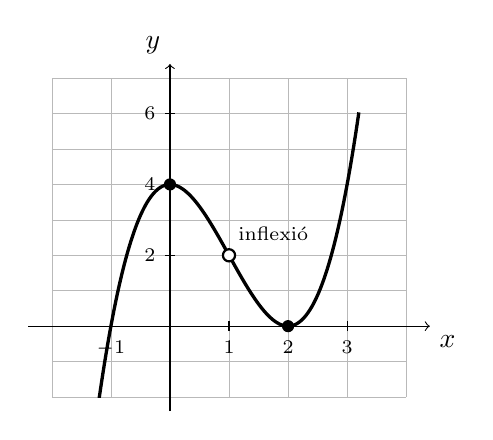
\begin{tikzpicture}[x=0.75cm,y=0.45cm]
  \draw[gray!55,very thin,step=1] (-2,-2) grid (4,7);
  \draw[->] (-2.4,0) -- (4.4,0) node[below right] {$x$};
  \draw[->] (0,-2.4) -- (0,7.4) node[above left] {$y$};
  \foreach \i in {-1,1,2,3} \draw (\i,0.15) -- (\i,-0.15) node[below,font=\scriptsize] {$\i$};
  \foreach \j in {2,4,6} \draw (0.08,\j) -- (-0.08,\j) node[left,font=\scriptsize] {$\j$};
  \begin{scope}
    \clip (-2,-2) rectangle (4,7);
    \draw[\colorgrafica,very thick,domain=-1.25:3.2,samples=120,smooth] plot (\x,{\x*\x*\x-3*\x*\x+4});
  \end{scope}
  \fill (0,4) circle (2.2pt); \fill (2,0) circle (2.2pt);
  \draw[fill=white,thick] (1,2) circle (2.2pt);
  \node[font=\scriptsize] at (1.75,2.6) {inflexió};
\end{tikzpicture}
\end{center}
\end{solucio}

\end{apartats}
